\documentclass[14pt]{extbook}
\usepackage{multicol, enumerate, enumitem, hyperref, color, soul, setspace, parskip, fancyhdr} %General Packages
\usepackage{amssymb, amsthm, amsmath, latexsym, units, mathtools} %Math Packages
\everymath{\displaystyle} %All math in Display Style
% Packages with additional options
\usepackage[headsep=0.5cm,headheight=12pt, left=1 in,right= 1 in,top= 1 in,bottom= 1 in]{geometry}
\usepackage[usenames,dvipsnames]{xcolor}
\usepackage{dashrule}  % Package to use the command below to create lines between items
\newcommand{\litem}[1]{\item#1\hspace*{-1cm}\rule{\textwidth}{0.4pt}}
\pagestyle{fancy}
\lhead{Progress Quiz 6}
\chead{}
\rhead{Version C}
\lfoot{9689-6866}
\cfoot{}
\rfoot{Spring 2021}
\begin{document}

\begin{enumerate}
\litem{
Construct the lowest-degree polynomial given the zeros below. Then, choose the intervals that contain the coefficients of the polynomial in the form $ax^3+bx^2+cx+d$.\[ \frac{-2}{5}, -6, \text{ and } \frac{4}{3} \]\begin{enumerate}[label=\Alph*.]
\item \( a \in [12, 19], b \in [72, 81], c \in [-96, -91], \text{ and } d \in [47, 50] \)
\item \( a \in [12, 19], b \in [72, 81], c \in [-96, -91], \text{ and } d \in [-54, -45] \)
\item \( a \in [12, 19], b \in [58, 66], c \in [-152, -146], \text{ and } d \in [47, 50] \)
\item \( a \in [12, 19], b \in [-79, -73], c \in [-96, -91], \text{ and } d \in [47, 50] \)
\item \( a \in [12, 19], b \in [-124, -115], c \in [159, 171], \text{ and } d \in [-54, -45] \)

\end{enumerate} }
\litem{
Describe the zero behavior of the zero $x = 4$ of the polynomial below.\[ f(x) = -6(x + 3)^{11}(x - 3)^{7}(x + 4)^{9}(x - 4)^{4} \]\begin{enumerate}[label=\Alph*.]
\begin{multicols}{2}\item 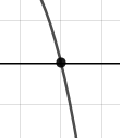
\includegraphics[width = 0.3\textwidth]{../Figures/polyZeroBehaviorAC.png}\item 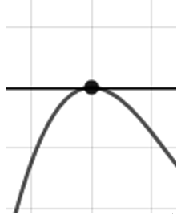
\includegraphics[width = 0.3\textwidth]{../Figures/polyZeroBehaviorBC.png}\item 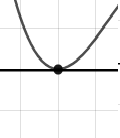
\includegraphics[width = 0.3\textwidth]{../Figures/polyZeroBehaviorCC.png}\item 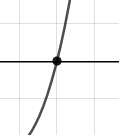
\includegraphics[width = 0.3\textwidth]{../Figures/polyZeroBehaviorDC.png}\end{multicols}\item None of the above.
\end{enumerate} }
\litem{
Which of the following equations \textit{could} be of the graph presented below?
\begin{center}
    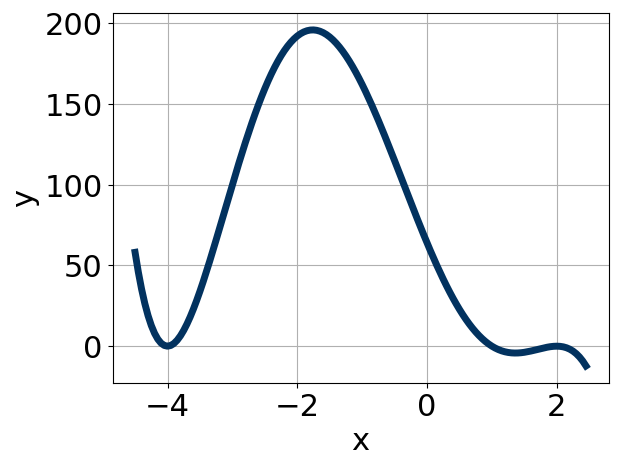
\includegraphics[width=0.5\textwidth]{../Figures/polyGraphToFunctionC.png}
\end{center}
\begin{enumerate}[label=\Alph*.]
\item \( 11x^{11} (x + 2)^{6} (x - 2)^{4} \)
\item \( -7x^{9} (x + 2)^{4} (x - 2)^{9} \)
\item \( -18x^{5} (x + 2)^{8} (x - 2)^{8} \)
\item \( 17x^{10} (x + 2)^{6} (x - 2)^{6} \)
\item \( -12x^{6} (x + 2)^{10} (x - 2)^{7} \)

\end{enumerate} }
\litem{
Describe the zero behavior of the zero $x = -3$ of the polynomial below.\[ f(x) = -6(x - 3)^{8}(x + 3)^{9}(x + 9)^{3}(x - 9)^{5} \]\begin{enumerate}[label=\Alph*.]
\begin{multicols}{2}\item 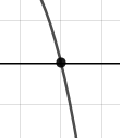
\includegraphics[width = 0.3\textwidth]{../Figures/polyZeroBehaviorCopyAC.png}\item 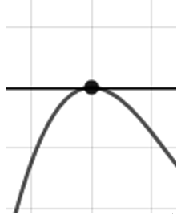
\includegraphics[width = 0.3\textwidth]{../Figures/polyZeroBehaviorCopyBC.png}\item 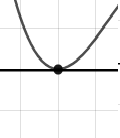
\includegraphics[width = 0.3\textwidth]{../Figures/polyZeroBehaviorCopyCC.png}\item 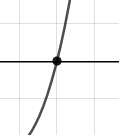
\includegraphics[width = 0.3\textwidth]{../Figures/polyZeroBehaviorCopyDC.png}\end{multicols}\item None of the above.
\end{enumerate} }
\litem{
Which of the following equations \textit{could} be of the graph presented below?
\begin{center}
    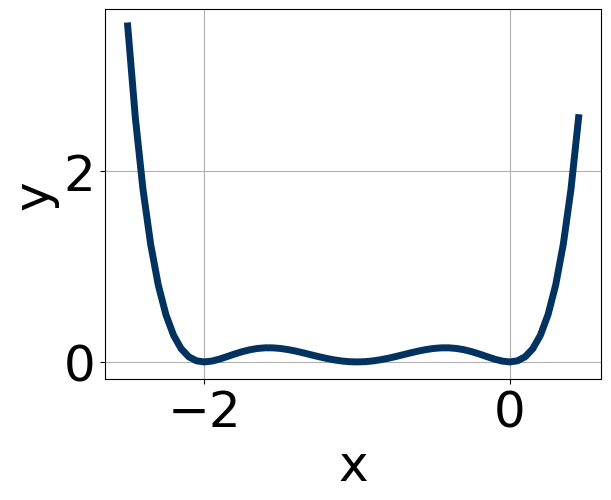
\includegraphics[width=0.5\textwidth]{../Figures/polyGraphToFunctionCopyC.png}
\end{center}
\begin{enumerate}[label=\Alph*.]
\item \( -4(x + 3)^{8} (x + 4)^{11} (x + 2)^{11} \)
\item \( -19(x + 3)^{8} (x + 4)^{10} (x + 2)^{6} \)
\item \( -4(x + 3)^{4} (x + 4)^{8} (x + 2)^{9} \)
\item \( 18(x + 3)^{10} (x + 4)^{6} (x + 2)^{6} \)
\item \( 2(x + 3)^{4} (x + 4)^{4} (x + 2)^{11} \)

\end{enumerate} }
\litem{
Describe the end behavior of the polynomial below.\[ f(x) = 3(x - 2)^{3}(x + 2)^{6}(x - 3)^{3}(x + 3)^{5} \]\begin{enumerate}[label=\Alph*.]
\begin{multicols}{2}\item 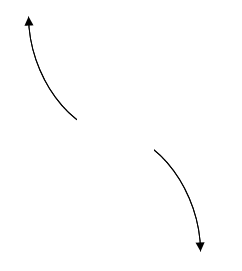
\includegraphics[width = 0.3\textwidth]{../Figures/polyEndBehaviorCopyAC.png}\item 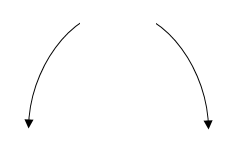
\includegraphics[width = 0.3\textwidth]{../Figures/polyEndBehaviorCopyBC.png}\item 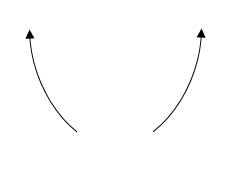
\includegraphics[width = 0.3\textwidth]{../Figures/polyEndBehaviorCopyCC.png}\item 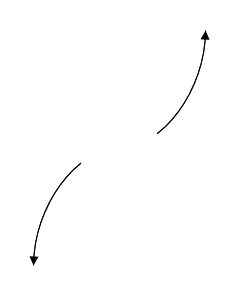
\includegraphics[width = 0.3\textwidth]{../Figures/polyEndBehaviorCopyDC.png}\end{multicols}\item None of the above.
\end{enumerate} }
\litem{
Construct the lowest-degree polynomial given the zeros below. Then, choose the intervals that contain the coefficients of the polynomial in the form $x^3+bx^2+cx+d$.\[ 4 + 5 i \text{ and } -2 \]\begin{enumerate}[label=\Alph*.]
\item \( b \in [-7, 0], c \in [24.91, 26.45], \text{ and } d \in [80.64, 83.45] \)
\item \( b \in [-1, 2], c \in [-3.56, -2.79], \text{ and } d \in [-10.45, -8.73] \)
\item \( b \in [2, 10], c \in [24.91, 26.45], \text{ and } d \in [-84.05, -81.44] \)
\item \( b \in [-1, 2], c \in [-2.86, -1.28], \text{ and } d \in [-9.04, -7.02] \)
\item \( \text{None of the above.} \)

\end{enumerate} }
\litem{
Describe the end behavior of the polynomial below.\[ f(x) = -4(x + 2)^{3}(x - 2)^{4}(x - 7)^{4}(x + 7)^{6} \]\begin{enumerate}[label=\Alph*.]
\begin{multicols}{2}\item 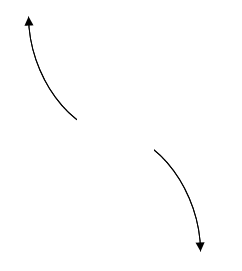
\includegraphics[width = 0.3\textwidth]{../Figures/polyEndBehaviorAC.png}\item 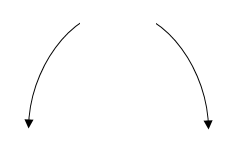
\includegraphics[width = 0.3\textwidth]{../Figures/polyEndBehaviorBC.png}\item 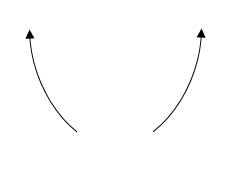
\includegraphics[width = 0.3\textwidth]{../Figures/polyEndBehaviorCC.png}\item 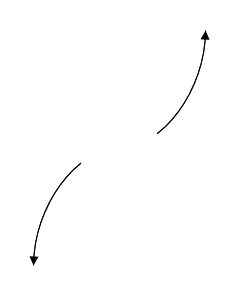
\includegraphics[width = 0.3\textwidth]{../Figures/polyEndBehaviorDC.png}\end{multicols}\item None of the above.
\end{enumerate} }
\litem{
Construct the lowest-degree polynomial given the zeros below. Then, choose the intervals that contain the coefficients of the polynomial in the form $x^3+bx^2+cx+d$.\[ 4 + 2 i \text{ and } -4 \]\begin{enumerate}[label=\Alph*.]
\item \( b \in [-4.2, -2.5], c \in [-14.9, -10.4], \text{ and } d \in [75, 81] \)
\item \( b \in [-1.7, 2.1], c \in [0.3, 5.3], \text{ and } d \in [-10, -2] \)
\item \( b \in [2.9, 6.9], c \in [-14.9, -10.4], \text{ and } d \in [-82, -79] \)
\item \( b \in [-1.7, 2.1], c \in [-0.5, 0.9], \text{ and } d \in [-20, -13] \)
\item \( \text{None of the above.} \)

\end{enumerate} }
\litem{
Construct the lowest-degree polynomial given the zeros below. Then, choose the intervals that contain the coefficients of the polynomial in the form $ax^3+bx^2+cx+d$.\[ 1, -5, \text{ and } \frac{-1}{3} \]\begin{enumerate}[label=\Alph*.]
\item \( a \in [-4, 5], b \in [18, 24], c \in [19, 24], \text{ and } d \in [3, 14] \)
\item \( a \in [-4, 5], b \in [11, 14], c \in [-15, -5], \text{ and } d \in [-9, 2] \)
\item \( a \in [-4, 5], b \in [-15, -12], c \in [-15, -5], \text{ and } d \in [3, 14] \)
\item \( a \in [-4, 5], b \in [-12, -6], c \in [-19, -14], \text{ and } d \in [-9, 2] \)
\item \( a \in [-4, 5], b \in [11, 14], c \in [-15, -5], \text{ and } d \in [3, 14] \)

\end{enumerate} }
\end{enumerate}

\end{document}